%!Tex Root = ../Tutorat2.tex
% ./Packete.tex
% ./Design.tex
% ./Deklarationen.tex
% ./Aufgabe1.tex
% ./Aufgabe3.tex
% ./Bonus.tex

\section{Task 2}

\setcounter{task}{1}

\begin{frame}[allowframebreaks]{Task 2}{Manual Scheduling\vspace{0.5cm}}
  \begin{itemize}
    \item We see from the table that the period P is 30, and we can use 3 as the frame f. Since this task set is a small one, we can derive a feasible schedule graphically...
      \begin{itemize}
        \item $P = lcm(15, 10, 6) = 30$
        \item for $f$ one does have the \alert{constraints}: \enquote{Is the period $P$ a multiple of the frame $f$}, $f \leq T_i, \forall$ tasks $\tau_i$, $f \geq C_i, \forall$ tasks $\tau_i$ and $2 f-\operatorname{gcd}\left(T_i, f\right) \leq D_i \forall$ tasks $\tau_i$ $\rightarrow 3$
        \item further steps are similiar to solving a \alert{Soduko}
      \end{itemize}
  \end{itemize}
  \begin{figure}
    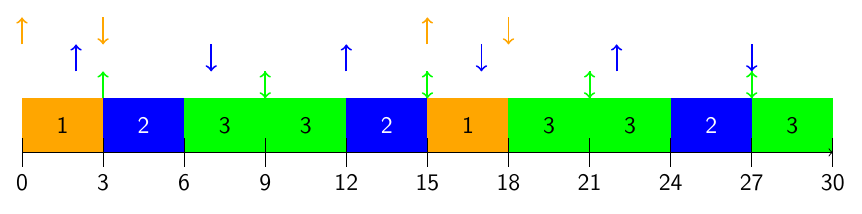
\includegraphics[width=0.7\paperwidth]{./figures/task2_schedule.png}
    \caption{Schedule for Task 2}
  \end{figure}
\end{frame}
